\documentclass{beamer}
   \usetheme{PaloAlto}
   % make math fonts look like article
   \usefonttheme[onlymath]{serif}
   \usepackage{algorithm2e}

   % Title page metadata
   \title[Neuro Fuzzy Hybridization]
   {A Neuro Fuzzy Hybridization Model for Nonlinear Control of a Fixed Wing UAV}
   \subtitle{Human-like Reasoning within Connectionist Structure}
   \author[Dadian]
   {\underline{Ohanes ~Dadian\inst{1}}\\
   Software Engineer\\
   Northrop Grumman}
   \subject{Computer Science}
\begin{document}
   \frame{\titlepage}

   \section{Topics}
   
   \begin{frame}
      \frametitle{Topics}
      \begin{itemize}
         \item Neuro Fuzzy Hybridization
         \item Fuzzy Logic
         \item Neural Networks
         \item Neuro Fuzzy Inference System (NFIS)
      \end{itemize}
   \end{frame}
   
   \section{Hybridization}

   \begin{frame}
      \frametitle{Neuro Fuzzy Hybridization}
      \begin{itemize}
         \item Neuro Fuzzy Hybridization is a hybrid-intelligent agent that combines a neural network with a fuzzy logic controller.
         \item The fuzzy logic controller provides human-like reasoning.
         \item The neural network provides learning and connectionist structure.
         \item Commonly referred to as neuro-fuzzy systems (NFS) or neuro-fuzzy inference systems (NFIS).
      \end{itemize}
   \end{frame}

   \section{Fuzzy Logic}

   \begin{frame}
      \frametitle{What is Fuzzy Logic?}
      \begin{itemize}
         \item Fuzzy logic is a form of many-valued logic.
         \begin{itemize}
            \item Many-valued logic is propositional calculus wthere consts of more than two truth tables.
            \item Truth tables of variables may be any real number between 0 and 1.
            \item Provides capability of deriving partial truth.
            \item Fuzzy logic was introduced in 1965 by Lofti Zadeh.
         \end{itemize}
         \item Came out of early research in fuzzy set theory.
         \item Dating back to the 1920s with Lukasiewicz and Tarski.
         \item Popular applications in control theory and artificial intelligence.
      \end{itemize}
   \end{frame}

   \begin{frame}
      \frametitle{Fuzzification}
      \begin{itemize}
         \item The following steps allow data to be fuzzified.
         \begin{itemize}
            \item Fuzzify all input values into fuzzy membership functions.
            \item Execute all applicable rules into the rulebase to compute fuzzy output functions.
            \item De-fuzzify the fuzzy output functions to get "crisp" output values.
         \end{itemize}
      \end{itemize}
   \end{frame}

   \begin{frame}
      \frametitle{Fuzzy Sets}
      \begin{columns}[T]
         \begin{column}[T]{5cm}
            \begin{itemize}
               \item These membership functions are paired with a set to form a Fuzzy Set, which are generally defined as traingle or trapezoid-shaped curve.
               \begin{itemize}
                  \item Each value has a slope where its value is increasing, peaking at 1, and a slope where the value is decreasing.
                  \item Can also be modeled as a sigmoid.
               \end{itemize}
            \end{itemize}
         \end{column}
         \begin{column}[T]{5cm}
            \begin{center}
               \underline{Logistic Sigmoid} \\
               $ x = \frac{e^{x}}{e^{x}+1} $ \\~\\
               \underline{Symmetric Property} \\
               $ S(x) + S(-x) =  1 $ \\~\\
               $ (S(x) + S(-x)) \times (S(y) + S(-y)) \times (S(z) + S(-z)) = 1 $ 
            \end{center}
         \end{column}
      \end{columns}
   \end{frame}

   \begin{frame}
      \frametitle{Fuzzy Logic Operators}
      \begin{columns}[T]
        \begin{column}[T]{5cm}
            \begin{itemize}
               \item Fuzzy logic works with membership values in a way that mimics boolean logic.
               \item These are generally adverbs such as very, or somewhat, which modify the meaning of a set using a mathematical formula.
               \item For TRUE/1 and FALSE/0, the fuzzy expressions produce the same result as the Boolean expressions.
            \end{itemize}
        \end{column}
        \begin{column}[T]{5cm}
            \begin{tabular}{| c | c |}
               \hline
               Boolean & Fuzzy \\
               \hline
               AND(x,y) & MIN(x,y) \\
               OR(x,y)  & MAX(x,y) \\
               NOT(x) & 1 - x \\
               \hline
            \end{tabular}
        \end{column}
      \end{columns}
   \end{frame}

   \begin{frame}
      \frametitle{Defuzzification}
      \begin{itemize}
         \item The goal is to get a continuous variable from fuzzy truth values.
         \item For each truth value, cut the membership function at this value
         \item Combine the resulting curves using the OR operator
         \item Find the center-of-weight of the area under the curve
         \item The x position of this center is then the final output.
      \end{itemize}
   \end{frame}

   \section{Neural Nets}
   
   \begin{frame}
      \frametitle{Neural Networks}
      \begin{itemize}
        \item A connectionist-based machine learning technique inspired by its biological counterpart.
            \begin{itemize}
               \item Connectionism dictates that nodes in a model are interconnected and perform in parallel.
               \item Contains linear input and output signals conjoined by a nonlinear hidden layer.
            \end{itemize}
         \item Learn new skills through example.
         \item No a priori knowledge.
            \begin{itemize}
               \item Relevant characteristics from learning material evolve over training.
            \end{itemize}
         \item Image Recognition is a prime example.
            \begin{itemize}
               \item Learn the skill for classifying images of dog.
                  \begin{itemize}
                     \item Use images of dogs labeled as "dog" or "not dog".
                     \item Build understanding of characteristics including tails, ears, fur, etc. over time.
                  \end{itemize}
            \end{itemize}
      \end{itemize}
   \end{frame}

   \begin{frame}
      \frametitle{Neural Networks contd.}
      \begin{columns}[T]
         \begin{column}[T]{5cm}
            \begin{itemize}
               \item The activation or transfer function generally comes in the form of a sigmoid, step, or linear combination function.
               \item Sigmoid is usually logistic or hyperbolic tangent.
            \end{itemize}
         \end{column}
         \begin{column}[T]{5cm}
            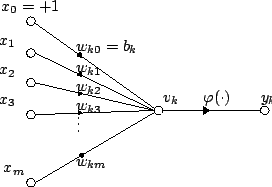
\includegraphics[height=2.8cm]{artificial_neuron}
                  \begin{center}
                     \underline{Logistic Sigmoid} \\
                     $ x = \frac{e^{x}}{e^{x}+1} $
                  \end{center}
                  \begin{center}
                     \underline{Hyperbolic Tangent} \\
                     $ x = \frac{1 - e^{-2x}}{1 + e^{-2x}} $
                  \end{center}
         \end{column}
      \end{columns}
   \end{frame}

   \begin{frame}
      \frametitle{Synapse}
      \begin{columns}[T]
         \begin{column}[T]{5cm}
            \begin{itemize}
               \item Synapses take the value of the input signal and multiply by its weight.
               \item The weight dictates the strength of the synapses connection between both neurons.
               \item Neurons sum all of the synapse fires and apply them to their activation function.
            \end{itemize}
         \end{column}
         \begin{column}[T]{5cm}
            \begin{figure}[htbp]
               \includegraphics[height=2.8cm]{synapse}
            \end{figure}
         \end{column}
      \end{columns}
   \end{frame}

   \begin{frame}
      \frametitle{Hidden Layer}
      \begin{columns}[T]
         \begin{column}[T]{5cm}
            \begin{itemize}
               \item Hidden Layers provide the ability of nonlinear learning.
               \begin{itemize}
                  \item Making sense of complicated problems using close approximations.
                  \item Allow contextualizing of such problems.
                  \item The use of multiple hidden layers provide the capability of deep learning.
                  \item They are deemed hidden, as they are not visible to the network output.
               \end{itemize}
               \item Circles represent neurons and lines represent synapses.
            \end{itemize}
         \end{column}
         \begin{column}[T]{5cm}
            \begin{figure}[htbp]
               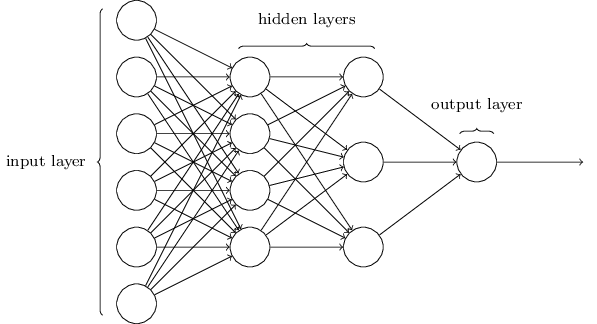
\includegraphics[height=2.8cm]{mlp-network}
            \end{figure}
         \end{column}
      \end{columns}
   \end{frame}

   \begin{frame}
      \frametitle{Learning}
      \begin{itemize}
         \item Neural nets are trained using a learning algorithm.
            \begin{itemize}
               \item Supervised Learning
                  \begin{itemize}
                     \item Maps an input value to an output value, based on labeled input-output pairs.
                     \item Used for speech and handwriting recognition.
                  \end{itemize}
               \item Unsupervised Learning
                  \begin{itemize}
                     \item Uncovering hidden structure from unlabeled data.
                     \item Used in biological classification and sequence analysis.
                  \end{itemize}
               \item Reinforcement Learning
                  \begin{itemize}
                     \item Taking actions within an environment, in order to maximize reward.
                     \item Used by robotic arms in manufacturing and financial trading.
                  \end{itemize}
            \end{itemize}
      \end{itemize}
   \end{frame}
   
   \begin{frame}
      \frametitle{Recurrent Neural Networks}
      \begin{columns}[T]
         \begin{column}[T]{5cm}
            \begin{itemize}
               \item A neural net where the synapses between neurons form a directed cycle.
               \item Signals traveling in both directions. 
               \item Output signal driven back into network to bias neurons for further training.
               \item Exhibits dynamic temporal behavior for a time sequence.
               \item Design can get quite complicated.
            \end{itemize}
         \end{column}
         \begin{column}[T]{5cm}
            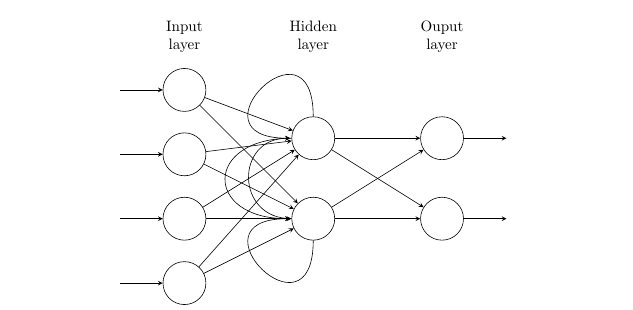
\includegraphics[height=3cm]{recurrent}
         \end{column}
      \end{columns}
   \end{frame}

   \section{ANFIS}

   \begin{frame}
      \frametitle{Artifical Neuro Fuzzy Inference System (ANFIS)}
      \begin{itemize}
         \item Provides a means of learning and adaptation.
         \item The Neural Network allows the Fuzzy Logic controller to be more systematic and less reliant on expert knowledge.
         \item The fuzzy inference system is trained using least square regression and gradient descent.
         \item The Neuro Fuzzy inference system is structured so that all possible situations may occur to the vehicle.
      \end{itemize}
   \end{frame}

   \begin{frame}
      \frametitle{ANFIS Architecture}
      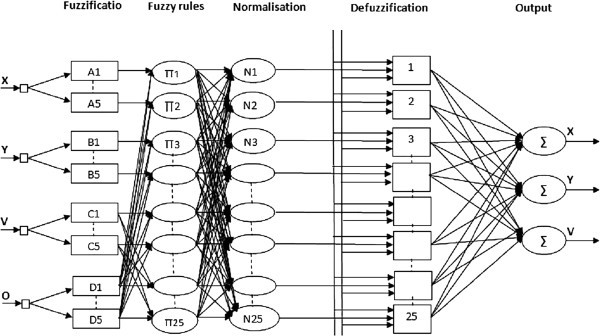
\includegraphics[height=6cm]{neuro_fuzzy_architecture}
   \end{frame}

   \begin{frame}
      \frametitle{Fuzzy Rule Set}
      \begin{algorithm}[H]
         \If{((x[1] = A[11]) \& (x[2] = A[12]) \& .. \&  (x[n] = A[1n]))}
         {
            f[1] = p[11] * x[1] + p[12] * x[2] + .. + x[n] * p[1n]
         } 
         \caption{Fuzzy Rule Set 1} 
      \end{algorithm}
      \begin{algorithm}[H]
         \If{((x[1] = A[21]) \&  (x[2] = A[22]) \& .. \& (x[n] = A[2n]))}
         {
            f[2] = p[21] * x[1] + p[22] * x[2] + .. + x[n] * p[2n]
         } 
         \caption{Fuzzy Rule Set 2} 
      \end{algorithm}
   \end{frame}

   \begin{frame}
      \frametitle{Fuzzy Rule Set, cont.}
      \begin{algorithm}[H]
         \If{((x[1] = A[m1]) \& .. \&  (x[n] = A[mn]))}
         {
            f[m] = p[m1] * x[1] + p[m2] * x[2] + .. + x[n] * p[mn]
         } 
         \caption{Fuzzy Rule Set M} 
      \end{algorithm}
   \end{frame}

   \begin{frame}
      \frametitle{Neural Architecture}
      \begin{itemize}
         \item 5 layers are employed.
         \item First layer introduces a  membership  function  in  universal  of  discourse  of  each input variable.
         \item Second layer represents the strength of the incentive of a rule.
         \item Third layer calculates the normalized output of each rule.
         \item Fourth layer where each node of this layer is an adaptive node of the node function.
         \item Layer five calculates all received signals and computes the linear output signal.
      \end{itemize}
   \end{frame}

   \begin{frame}
      \frametitle{Learning}
      \begin{itemize}
         \item Hybrid Learning is used a train the ANFIS.
         \item Combines least squares regression and gradient decent.
      \end{itemize}
   \end{frame}
   
   \begin{frame}
      \frametitle{Training for PID Tuning}
      \begin{itemize}
         \item Validated flight dynamics model for the UAV will be used to generate input-output data.
         \item The simulated data (roll, pitch, yaw) will be then used for train the ANFIS model.
         \item On-line training was then performed to correct for the inversion errors.
         \item Data required for the on-line training was obtained from FlightGear model of the aircraft in software-in-the-loop simulation.
      \end{itemize}
   \end{frame}
   
   \begin{frame}
      \frametitle{Flight Simulation using FlightGear}
      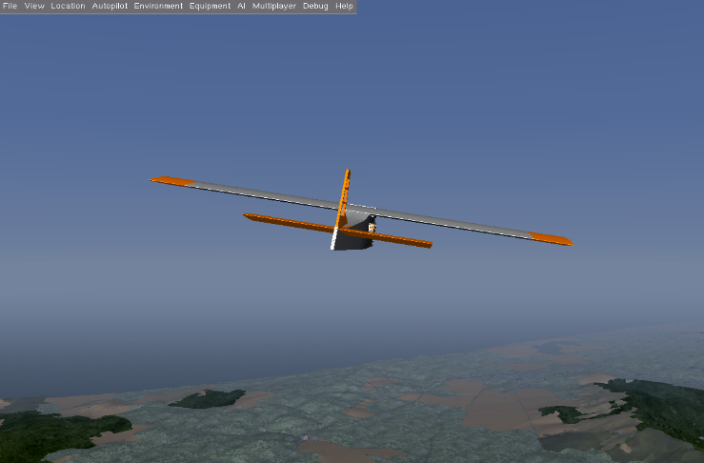
\includegraphics[height=6cm]{flightgear}
   \end{frame}

   \begin{frame}
      \frametitle{Prototyping Platform}
      \begin{columns}[T]
         \begin{column}[T]{5cm}
            \begin{itemize}
               \item 16-core Epiphany RISC SOC
               \item Zynq SOC (FPGA + ARM A9)
               \item Gigabit Ethernet
               \item 1GB SDRAM
               \item Micro-SD storage
               \item Up to 48 GPIO pins
            \end{itemize}
         \end{column}
         \begin{column}[T]{5cm}
            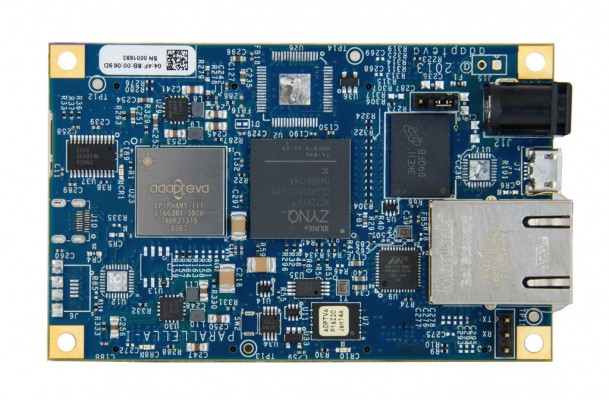
\includegraphics[height=3.7cm]{parallela}
         \end{column}
      \end{columns} 
   \end{frame}

   \section{Conclusion}
 
   \begin{frame}
      \frametitle{Conclusion}
      \begin{itemize}
         \item Hybridization model can successfully perform identification and nonlinear control of UAVs.
         \item Able to perform both offline and online learning.
         \item Offline training allows for inversion of feedback linearization to be computed.
         \item Simulation showed controller performance significantly improved in both open and closed loop responses.
         \item ESN facilitated adaptability with more ease than a feed forward network.
         \item Able to decrease delta of MSE with less training iterations.
         \item Shorter bursts and Lyapunov stable.
      \end{itemize}
   \end{frame}

   \section{Q \& A}

   \begin{frame}
      \frametitle{Q \& A}
   \end{frame}
\end{document}
